\section{Détermination des courbes en S}

Nous avons voulu modéliser dans cette partie la condition d'équilibre thermique du plan équatorial du disque d'accrétion c'est-à-dire représenter l'état du système lorsque la quantité de chaleur produite ($Q^+$)est égale à la quantité de chaleur dissipée ($Q^-$), lorsque le terme de refroidissement est égal au terme de chauffage.
\begin{equation}
Q^+ = Q^-
\end{equation}
L'équation thermique devient donc, en négligeant le terme d'advection ($Q_{adv}$) qui représente la chaleur apportée ou emportée par la matière en mouvement.
\begin{equation}
Cv\frac{\partial T}{\partial t} = 0
\end{equation}
avec $Cv$ la capacité calorifique à volume constant par unité de masse du mélange de gaz et de radiation que l'on peut réécrire
\begin{equation}
\frac{\partial T}{\partial t} = 0
\end{equation}
Cette équation est stationnaire, elle ne dépend pas du temps mais elle dépend de la distante par rapport au centre du disque. Nous avons donc dû générer 256 courbes en S différentes pour chaque position du disque.

Nous avons voulu représenter sur un même graphique l'évolution de la température en fonction de densité de surface, c'est à dire représenter la fonction T($\Sigma$).
\\   

\subsection{Etablissement de la fonction}

Au premier abord, pour obtenir une seule courbe en S, le rayon r a été fixé. Ainsi la vitesse angulaire $\Omega$ a été préalablement définie. Par la suite nous avons répété la démarche suivante pour 256 différentes valeurs du rayon.
\\
En première partie, nous avons calculé la demi-hauteur H en utilisant la résolution d' une équation quadratique ne dépendant que de (T,$\Sigma,\Omega$) (Voir \ref{Equation}).
\\
Ensuite, la densité volumique $\rho$, la vitesse du son $c_s$ et la viscosité $\nu$. 
\\
De plus $\kappa_{ff}$, $\kappa_{e}$ et $\epsilon_{ff}$ pour pouvoir calculer le flux radiatif $F_z$ et déduire la différence des deux termes de chaleurs (en ne prenant pas en compte le terme d' advection) :
\\
\begin{equation} 
\label{eq:qplus-qmoins}
Q^+ - Q^- = 0. 
\end{equation}
\\
Nous avons aussi déterminé la profondeur optique effective $\tau_{eff}$. Selon sa valeur, nous pouvons nous placer dans un cas dit optiquement épais ($\tau_{eff} > 1$) ou bien dans le cas optiquement mince  ($\tau_{eff} < 1$).
Cependant nous ne l' avons pas utilisé comme critère pour le choix de l' expression du flux pour éviter de tomber sur des solutions stables artificielles qui seraient le fruit d' interpolations aux alentours de $\tau_{efff}$ = 1 où a lieu le basculement entre les deux approximations utilisées. 
\\
Nous avons donc calculé \ref{eq:qplus-qmoins} dans deux cas où on a imposé l' expression du flux radiatif. Ainsi, nous avons un algorithme où l' on peut fixer les valeurs de T et $\Omega$ pour obtenir une fonction ne dépendant que de $\Sigma$.

\subsection{Intervalle de température}
La résolution de la courbe en S nécessite de se placer dans un intervalle de température relativement restreint correspondant à la valeur de basculement de $\tau$ entre le cas optiquement épais et le cas optiquement mince.
Pour avoir un premier ordre de grandeur, nous nous sommes basés sur l'équation donnant la luminosité d'Eddington \ref{eq::} puis celle permettant de définir le taux d'accretion critique \ref{eq::} qui nous a donné la valeur de la température caractéristique $T_0$ de $1,40.10^6$ K. Nous avons ensuite, par paliers successifs, déterminé les intervalles de température permettant de représenter ce basculement d'état. Les deux valeurs que nous avons prises sont : $T_{min}$ = 2,94.$10^5 K$ et $T_{max}$ 6,2.$10^6 K$ 
\\


\subsubsection{Méthode de la dichotomie}

Pour déterminer la densité de surface associée à une valeur de température précise, nous avons procédé par dichotomie.
Cette méthode consiste à trouver les coordonnées où s' annule une fonction continue en partant d' un intervalle de départ et en le divisant successivement pour cerner l' intervalle le plus petit possible où se trouve la solution.  
\\
Soit f(T,$\Sigma$) = $Q^+$ - $Q^-$ = 0,  une fonction continue et strictement monotone dans un intervalle [$\Sigma_{min}$ ; $\Sigma_{max}$] pour un T donné. Si f(T,$\Sigma_{min}$ ) et  f(T,$\Sigma_{max}$ ) sont de signes opposés, alors d' après le théorème de la bijection il existe une solution unique comprise dans cette intervalle. 
\\
Nous avons appliqué cette bissection en divisant à chaque fois l' intervalle en deux jusqu' à obtenir une solution avec une précision de $10^-6$ et en limitant le nombre d' itérations pour des raisons pratiques. Nous avons alors obtenu deux graphes, représentant T en fonction de $\Sigma$ pour un milieu optiquement épais (tracé courbé) et pour un milieu optiquement mince (relation linéaire).
\\

\begin{figure}[htb!]
\centering
\begin{tabular}{cc} 
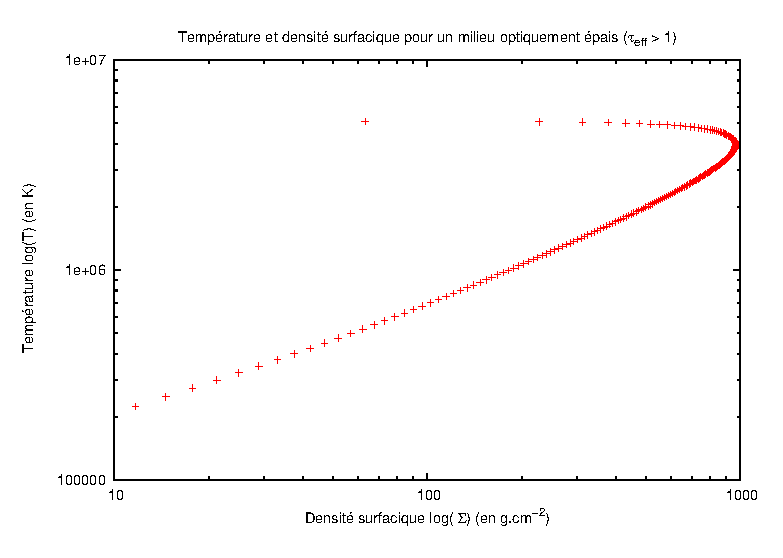
\includegraphics[height=0.3\textwidth]{S_curve_thick.eps} &
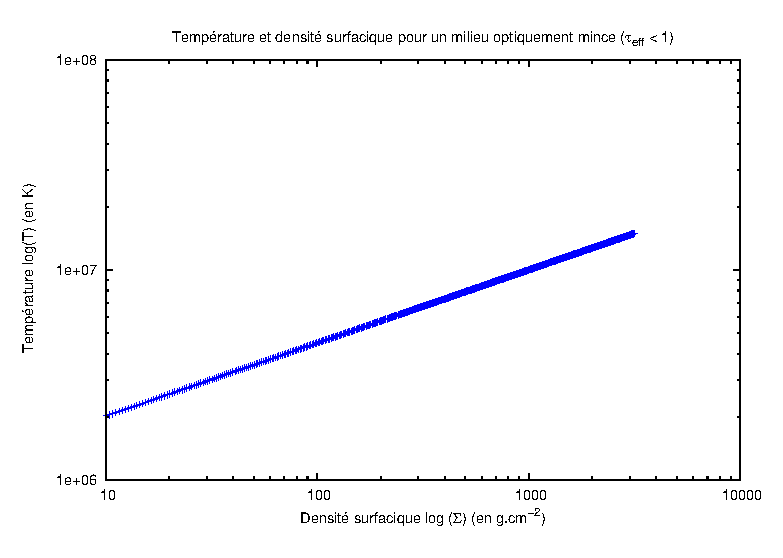
\includegraphics[height=0.3\textwidth]{S_curve_thin.eps} \\
\end{tabular}
  \caption{Cas optiquement épais (gauche) et optiquement mince (droite)}
\label{Fig::}
\end{figure}




\subsubsection{Méthode de Brent}
La méthode de Brent est une méthode de recherche de "zéros" d'une fonction combinant les méthodes de la dichotomie, de la sécante et l'interpolation quadratique inverse pour en utiliser tous leurs avantages. La méthode de l'interpolation quadratique inverse est une méthode de convergence rapide (ordre 2).
\begin{equation}
f(b) \ne f(a) \text{ et } f(b) \ne f(c) 
\end{equation}
Nous utilisons la méthode de l'interpolation quadratique inverse.
\begin{equation}
x = \frac{(y-f(a)(y-f(b))c}{(f(c)-f(a))(f(c)-f(b))} + \frac{(y-f(b)(y-f(c))a}{(f(a)-f(b))(f(a)-f(c))} +  \frac{(y-f(c)(y-f(a))b}{(f(b)-f(c))(f(b)-f(a))}
\end{equation}
Sinon, nous utilisons la méthode de la sécante vue précédemment. Si la méthode de la sécante n'est pas efficace \footnote{C'est à dire.....}, nous utilisons la méthode de la dichotomie.
\\
\subsubsection{Méthodes alternatives à la dichotomie}
La méthode de la dichotomie est une méthode simple et robuste pour trouver les "zéros" d'une fonction mais elle demande un grand nombre de d'itérations. En effet cette méthode converge linéairement.
\\
%%%%[A VERIFIER]
Le nombre d'itérations par une méthode de dichotomie est donnée par la formule suivante : 
\begin{equation}
n = \frac{log(borne_{sup} - borne_{inf}) + log(\epsilon)}{log(2)} 
\end{equation}

Nous avons donc regardé s' il existait des méthodes qui convergeaient plus rapidement et de manière tout aussi robuste. 

\subsubsection{Méthode de Newton}
La méthode de Newton parfois appelée méthode de Newton-Raphson, décrite dans le \textit{De analysi per aequationes numero terminorum infinitas} en 1669.

\begin{equation}
x_{k+1} = x_k - \frac{f(x_k)}{f'(x_k)}
\end{equation}

Convergence quadratique...

Cependant il faut que f soit de classe $C^1$
\\

\subsubsection{Méthode de la sécante}

Un des gros inconvénient de la méthode de Newton est d'avoir à calculer la dérivée de la fonction. La méthode de la sécante permet de contourner cet obstacle ne nécessite pas que la fonction soit de classe $C^1$


\begin{equation}
x_{n+1} = x_n - \frac{x_n - x_{n-1}}{f(x_n) - f(x_{n-1})}
\end{equation}

Cette méthode converge plus rapidement que la méthode de la dichotomie mais moins rapidement que la méthode de Newton (son ordre de convergence est compris entre 0 et 1 \footnote{Pour être plus précis l'ordre de convergence de cette méthode est égale à $\frac{1 + \sqrt{5}}{2}$} qui est le nombre d'or.). Elle permet également de s'affranchir également de la contrainte de l'intervalle de la fonction de la dichotomie. En revanche, cette méthode peut ne pas être robuste si la valeur initial est trop éloignée de la solution ou s'il existe des racines multiples.

\begin{figure}[htb!]
	\centering
	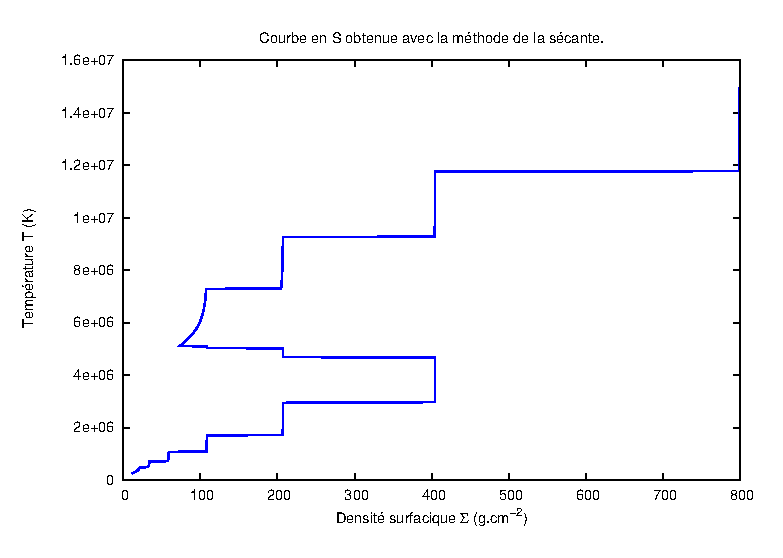
\includegraphics[height=0.7\textwidth]{S_curve_secant.eps}
	\caption{méthode de la sécante}
	\label{Fig::bench}
\end{figure}
%\FloatBarrier


\subsubsection{Autres méthodes}


\subsection{Comparaison des différentes méthodes}

\begin{figure}[htb!]
	\centering
	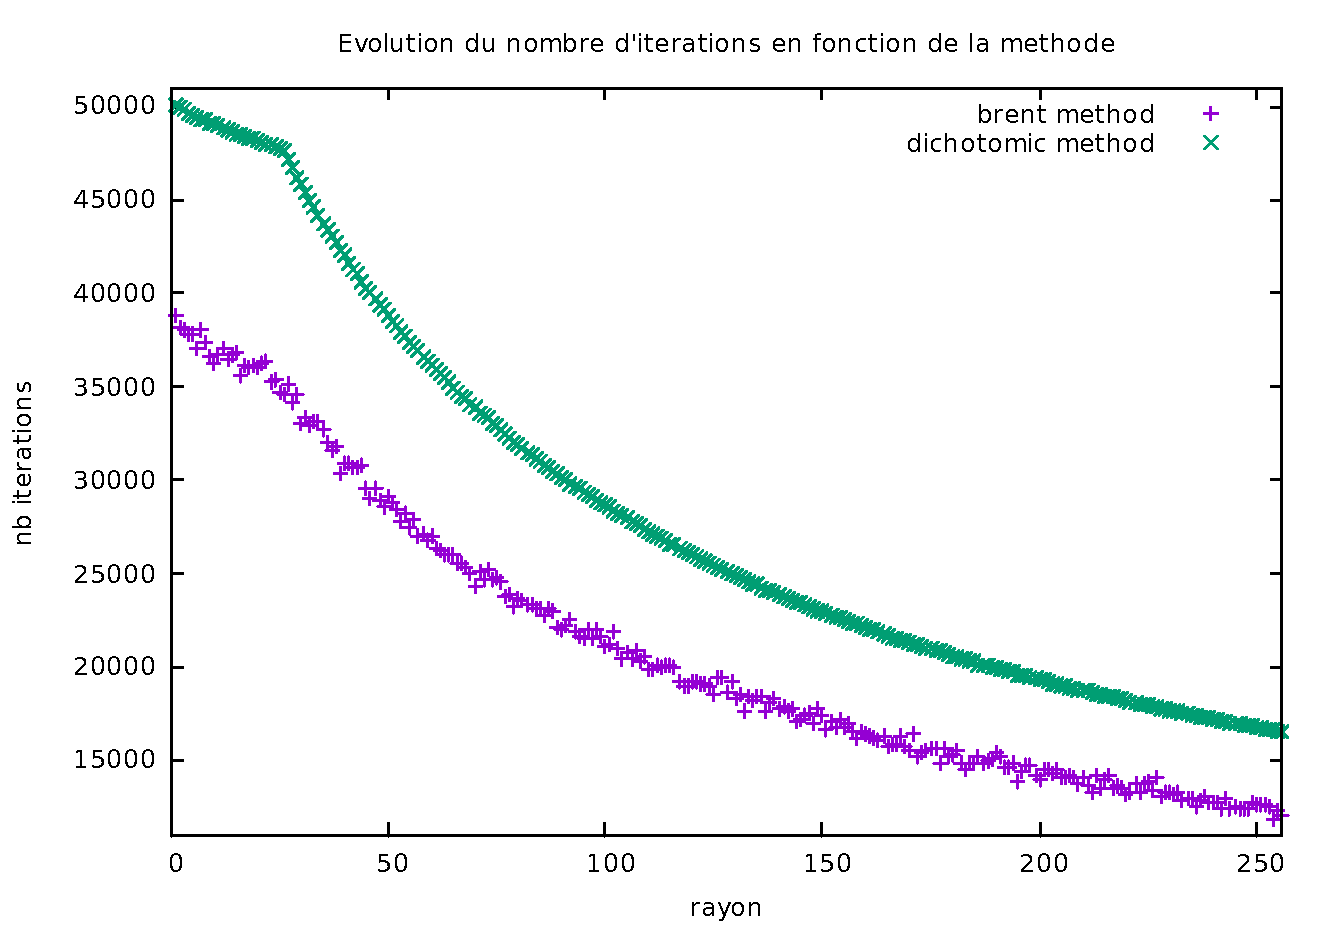
\includegraphics[height=0.5\textwidth]{brent_method3.pdf}
	\caption{Comparaison du nombre d'itérations nécessaire pour converger pour la méthode de la dichotomie et celle de Brent.}
	\label{Fig::bench}
\end{figure}


\subsection{Détermination des points critiques}
Afin de déterminer la propagation de l' instabilité thermique, il faut trouver le point critique où le système devient instable. Au niveau de la courbe en S, ceci a lieu sur la branche inférieure au niveau de la courbure : au-delà de ce point la densité surfacique diminue tandis que la température continue à s' élever. Sur la figure \ref{Fig::stable} la zone d'instabilité est représentée en bleue.

\begin{figure}[htb!]
	\centering
	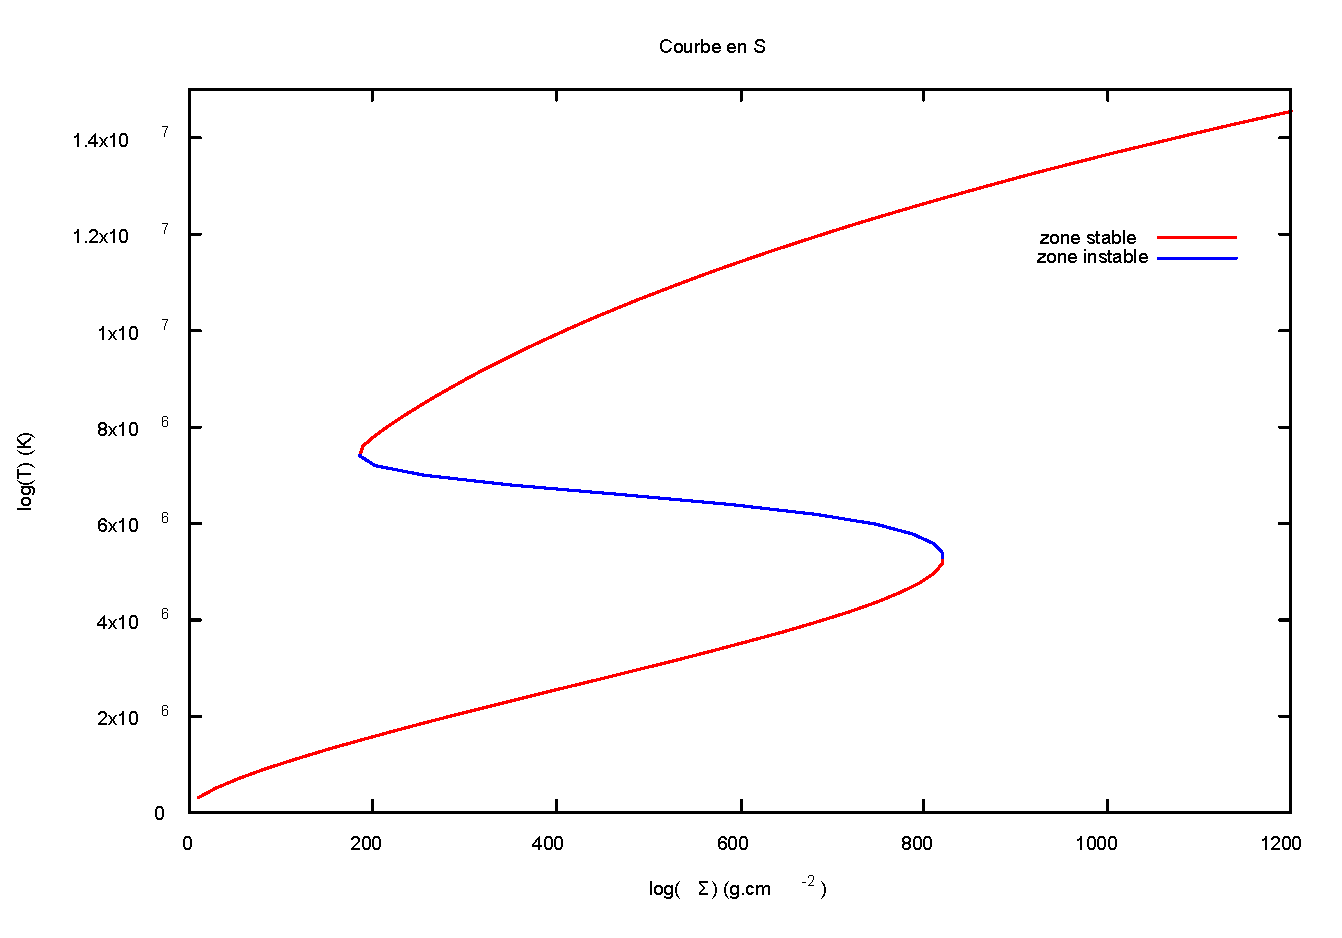
\includegraphics[height=0.7\textwidth]{stable.pdf}
	\caption{Zones stables et instables de la courbe en S}
	\label{Fig::stable}
\end{figure}
%\FloatBarrier

Pour trouver les coordonnées de ce point critique, nous avons comparé les valeurs de $\Sigma$ (calculé pour un milieu optiquement épais) pour chaque point en augmentant T. Lorsque la variation de la courbe change, c' est-à-dire quand $\Sigma$ cesse d' augmenter et commence à diminuer, nous avons repéré les coordonnées du dernier point pour lequel la densité surfacique croît.  
\\
Dans le code, nous avons nommé "deuxième point critique", le point où a lieu le basculement d'épaisseur optique. Sur les graphes, ce point se situe à l' intersection des deux branches et signale le changement de régime où on a utilisé une approximation de diffusion à une autre approximation où l'on doit prendre en compte les pertes par rayonnement de freinage (le refroidissement par bremsstrahlung).
\\
Pour le repérer, nous avons eu la même approche que pour pour le point d' instabilité trouvé préalablement. Cette fois-ci, nous avons comparé le $\Sigma$ déterminé pour un milieu optiquement épais à celui optiquement mince. Quand le premier devient plus petit que le second, celà signifie que la densité surfacique arrête de décroître et qu' elle commence à augmenter linéairement en fonction de la température. 
\\
%%%%%%%%[courbe en S avec les points légendés + ?evolution en fonction de r ?]

\subsection{Construction de la courbe}

En combinant les points trouvés dans le cas optiquement épais jusqu'au deuxième point critique et les points trouvés dans le cas optiquement mince, nous avons pu assembler les deux parties de la courbe en S.

\begin{figure}[htb!]
	\centering
	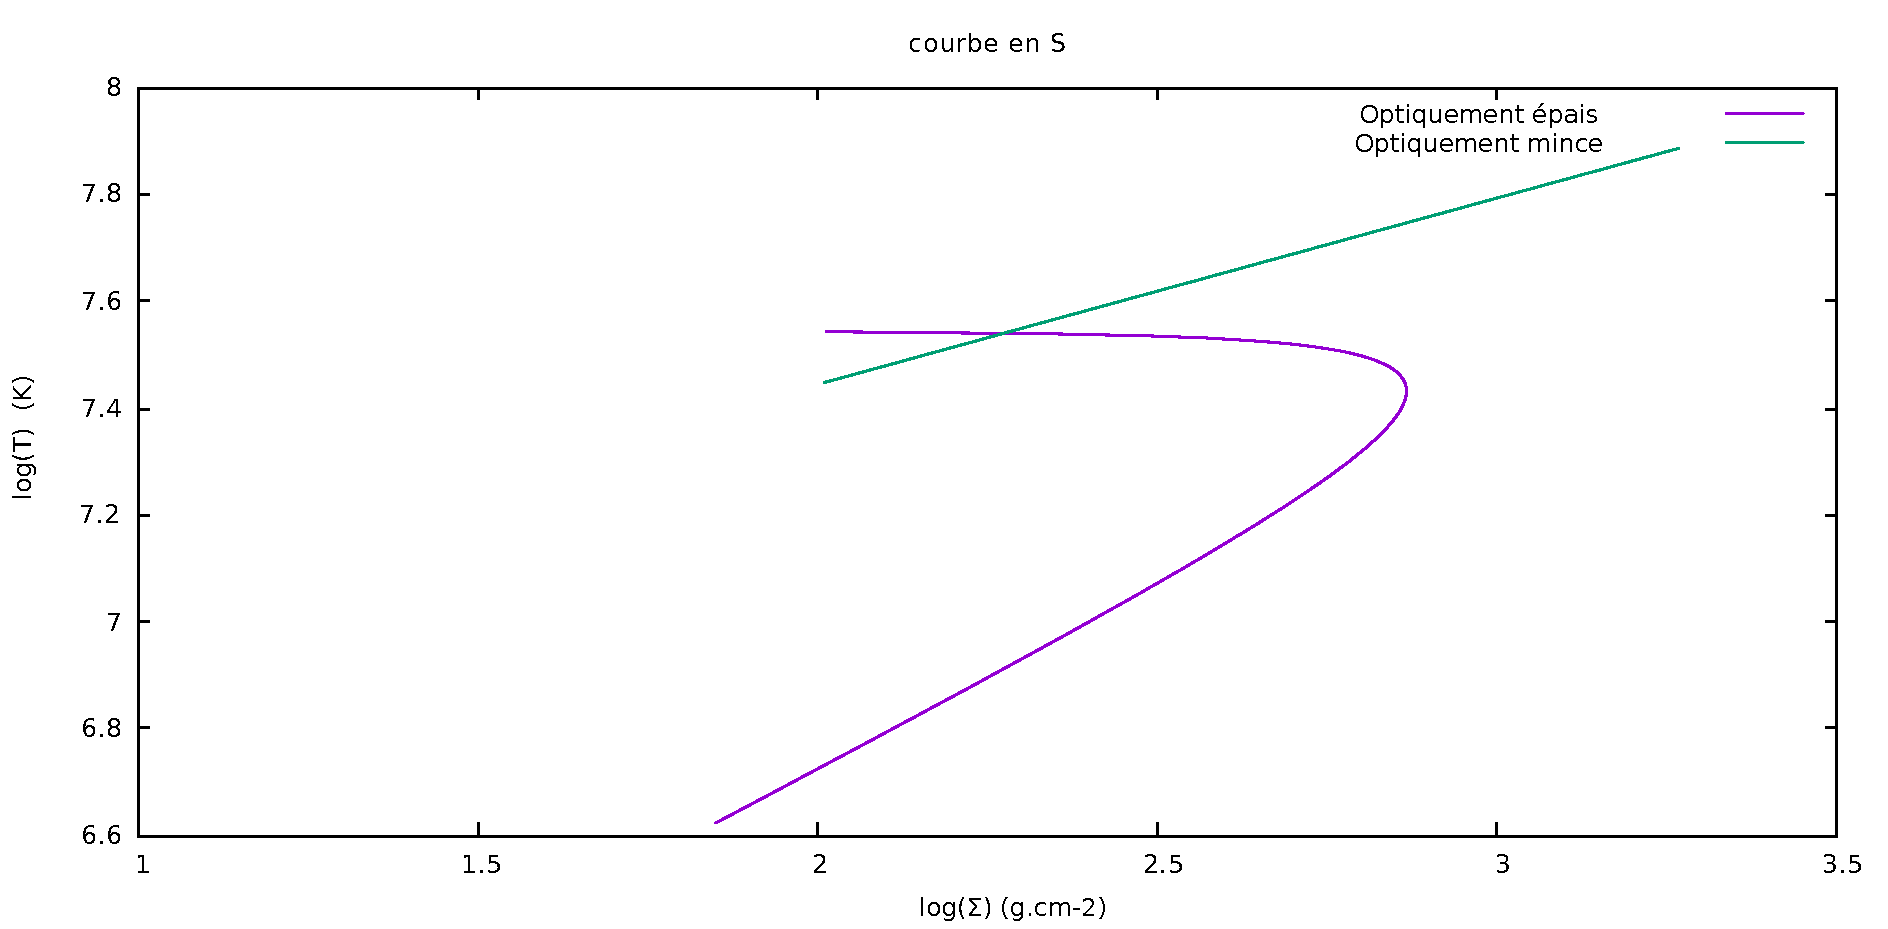
\includegraphics[height=0.5\textwidth]{deux_parties.pdf}
	\caption{Construction de la courbe en S}
	\label{Fig::bench}
\end{figure}


Nous avons donc pour chaque rayon une courbe en S représenté sur le graphe ci-dessous.
\begin{figure}[htb!]
	\centering
	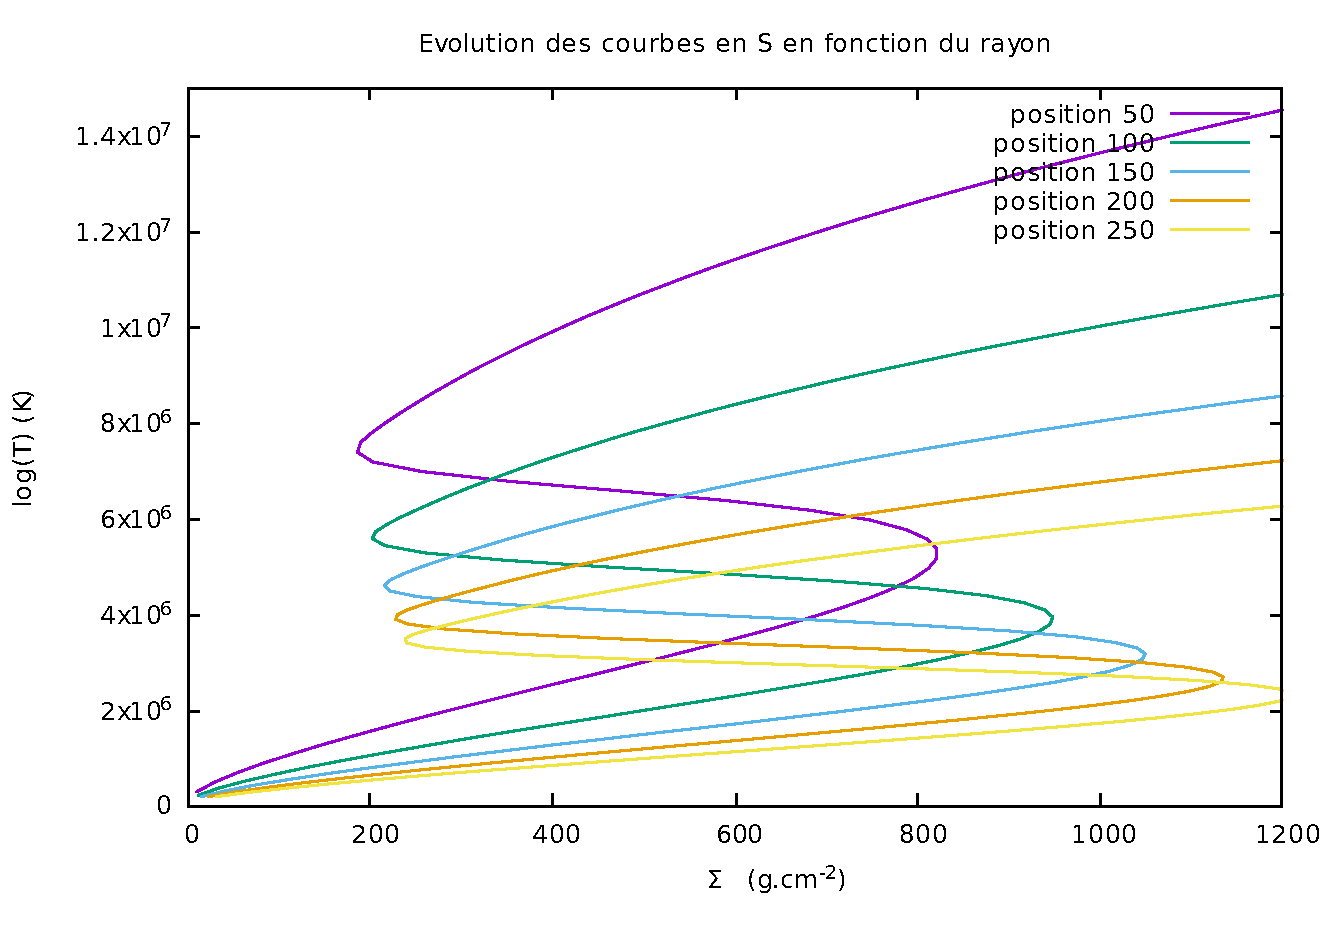
\includegraphics[height=0.7\textwidth]{evolutioncourbes.pdf}
	\caption{Evolution de la courbe en S en fonction de la distance au centre}
	\label{Fig::bench}
\end{figure}



\subsection{Evolution du $\tau_eff$}

D' après nos calculs nous trouvons un $\tau_eff$ aux alentours de 0,06 lors de la transition d'un milieu dit optiquement épais à un milieu optiquement mince. Cette valeur ne correspond pas à la valeur théorique où $\tau_eff$ = 1. 
Celà pose un problème au niveau de la partie d'intégration car notre branche linéaire est translatée par rapport à celle définie par la théorie. 
Cette différence de valeurs peut être expliquée par une erreur au niveau de l’adimensionnement ou bien dans les équations que nous avons utilisées ainsi que peut-être par une faute cachée dans nos paramètres ou nos constantes. 
\\
En fonction du rayon r, les coordonnées dans l' espace {T,$\Sigma$} des points ayant une valeur critique de $\tau_eff$ semblent évoluer de manière à ce que la température diminue et la densité surfacique augmente.
%%%manque d'inspiration  

\begin{figure}[htb!]
	\centering
	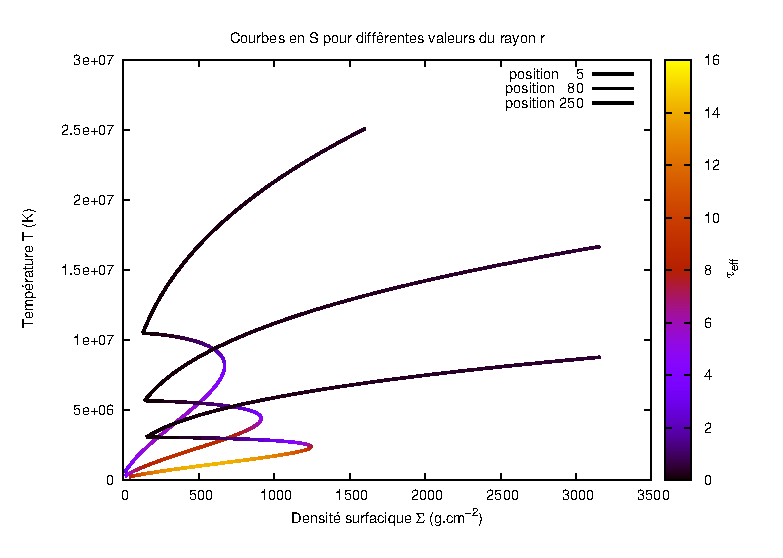
\includegraphics[height=0.7\textwidth]{S_curves_tau.eps}
	\caption{\textit{Evolution de la profondeur optique de la courbe en S pour diffèrents rayons.}  }
	\label{Fig::bench}
\end{figure}

\subsection{Idées avortées}
\begin{enumerate}

\item Calcul direct $Q^+ = Q^-$
\\
Pour définir la température T en fonction de $\Sigma$, nous avons d' abord essayé de simplifier l' égalité $Q^+ = Q^-$ , qui traduit l' équilibre thermique local, en remplaçant tous les termes par T,$\Sigma$ et $\Omega$. Cela donne deux expressions (selon l'opacité du milieu) de fonctions implicites où ces variables sont couplées.
La résolution n' étant pas plus simple qu' avant le changement et afin d' éviter toute erreur induite lors du remplacement des différentes variables impliquées, nous avons préféré de calculer indépendamment chaque variable dans un ordre bien choisi. 
\\

\item Calcul des points critiques par dérivation de la fonction T($\Sigma$)
Comme nous n'avions pas à notre disposition une expression explicite d' allure T = f($\Sigma$), la dérivation des solutions issues d' une série d'équations ne semblait pas l'approche la plus efficace pour trouver le point critique d' instabilité. De plus, en dérivant nous aurions eu un problème au niveau du deuxième point critique qui est un point anguleux.
\end{enumerate}

